\documentclass[border=6pt]{standalone}
\usepackage{tikz,amsmath,amssymb}
\usetikzlibrary{arrows.meta,positioning,calc,fit,backgrounds}
\definecolor{cres}{HTML}{DBEAFE}\definecolor{cresb}{HTML}{1D4ED8}
\definecolor{catt}{HTML}{FDE68A}\definecolor{cattb}{HTML}{B45309}
\definecolor{cconv}{HTML}{E5E7EB}\definecolor{cconvb}{HTML}{374151}
\definecolor{cemb}{HTML}{DCFCE7}\definecolor{cembb}{HTML}{15803D}
\definecolor{cskip}{HTML}{7C3AED}\definecolor{cio}{HTML}{FCE7F3}\definecolor{ciob}{HTML}{BE185D}
\begin{document}
\sffamily\scriptsize
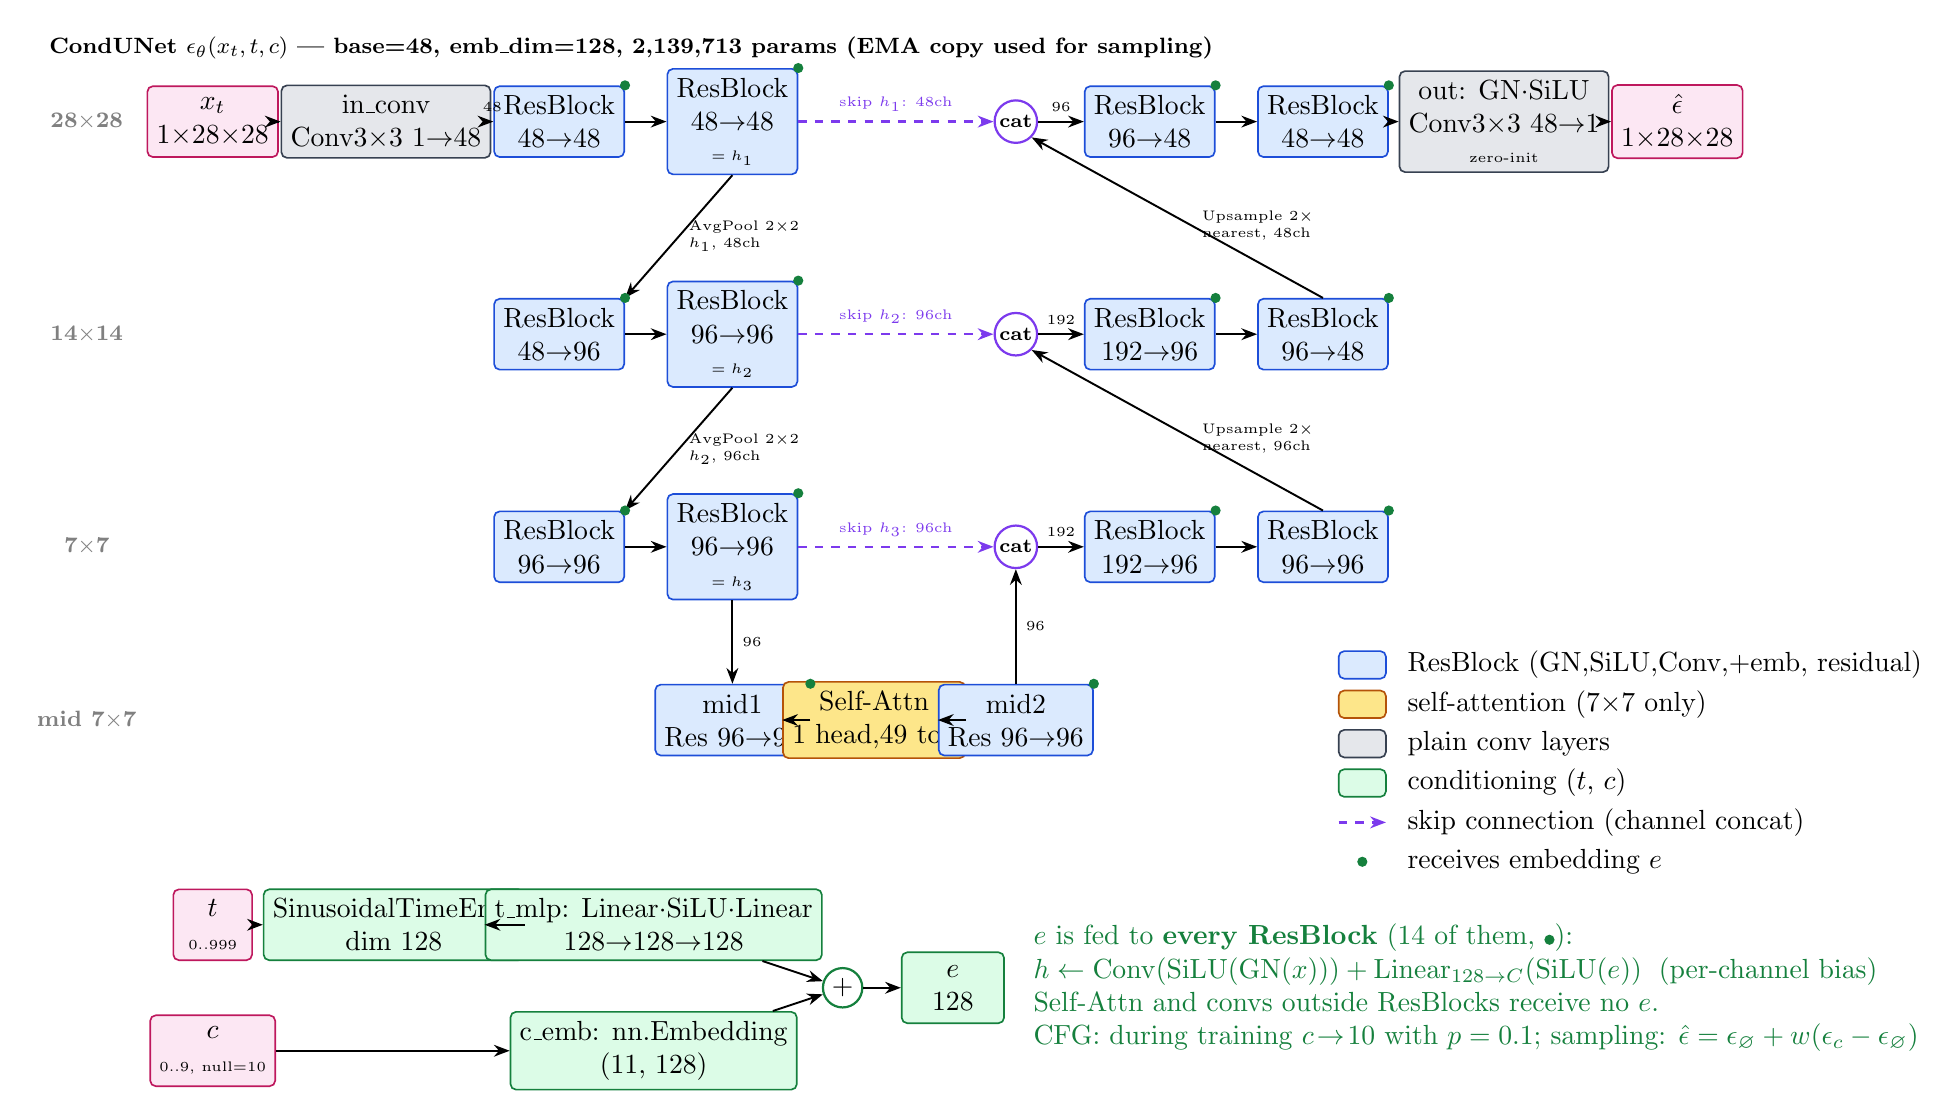
\begin{tikzpicture}[
  >={Stealth[length=2mm]},
  blk/.style={draw,rounded corners=2pt,minimum width=16mm,minimum height=9mm,align=center,line width=.6pt},
  res/.style={blk,fill=cres,draw=cresb},
  att/.style={blk,fill=catt,draw=cattb},
  cnv/.style={blk,fill=cconv,draw=cconvb},
  emb/.style={blk,fill=cemb,draw=cembb},
  io/.style={blk,fill=cio,draw=ciob,minimum width=15mm},
  cat/.style={circle,draw=cskip,fill=white,line width=.8pt,inner sep=1pt,font=\bfseries\scriptsize},
  dot/.style={circle,fill=cembb,inner sep=1.3pt},
  lvl/.style={font=\bfseries\footnotesize,text=gray},
  flow/.style={->,line width=.7pt},
  skipa/.style={->,line width=.9pt,draw=cskip,dashed},
]
% ---------- level 28 ----------
\node[lvl] at (-1.6,0) {28$\times$28};
\node[io]  (x)   at (0,0)    {$x_t$\\1$\times$28$\times$28};
\node[cnv] (in)  at (2.2,0)  {in\_conv\\Conv3$\times$3 1$\to$48};
\node[res] (d10) at (4.4,0)  {ResBlock\\48$\to$48};
\node[res] (d11) at (6.6,0)  {ResBlock\\48$\to$48\\[-1pt]{\tiny $=h_1$}};
\node[cat] (c1)  at (10.2,0) {cat};
\node[res] (u10) at (11.9,0) {ResBlock\\96$\to$48};
\node[res] (u11) at (14.1,0) {ResBlock\\48$\to$48};
\node[cnv] (out) at (16.4,0) {out: GN$\cdot$SiLU\\Conv3$\times$3 48$\to$1\\[-1pt]{\tiny zero-init}};
\node[io]  (eps) at (18.6,0) {$\hat\epsilon$\\1$\times$28$\times$28};
% ---------- level 14 ----------
\node[lvl] at (-1.6,-2.7) {14$\times$14};
\node[res] (d20) at (4.4,-2.7) {ResBlock\\48$\to$96};
\node[res] (d21) at (6.6,-2.7) {ResBlock\\96$\to$96\\[-1pt]{\tiny $=h_2$}};
\node[cat] (c2)  at (10.2,-2.7) {cat};
\node[res] (u20) at (11.9,-2.7) {ResBlock\\192$\to$96};
\node[res] (u21) at (14.1,-2.7) {ResBlock\\96$\to$48};
% ---------- level 7 ----------
\node[lvl] at (-1.6,-5.4) {7$\times$7};
\node[res] (d30) at (4.4,-5.4) {ResBlock\\96$\to$96};
\node[res] (d31) at (6.6,-5.4) {ResBlock\\96$\to$96\\[-1pt]{\tiny $=h_3$}};
\node[cat] (c3)  at (10.2,-5.4) {cat};
\node[res] (u30) at (11.9,-5.4) {ResBlock\\192$\to$96};
\node[res] (u31) at (14.1,-5.4) {ResBlock\\96$\to$96};
% ---------- bottleneck ----------
\node[lvl] at (-1.6,-7.6) {mid 7$\times$7};
\node[res] (m1) at (6.6,-7.6)  {mid1\\Res 96$\to$96};
\node[att] (at) at (8.4,-7.6)  {Self-Attn\\1 head,49 tok};
\node[res] (m2) at (10.2,-7.6) {mid2\\Res 96$\to$96};
% ---------- main flow ----------
\draw[flow] (x)--(in); \draw[flow] (in)--node[above,font=\tiny]{48}(d10); \draw[flow] (d10)--(d11);
\draw[flow] (d11.south) -- node[right,align=left,font=\tiny]{AvgPool 2$\times$2\\$h_1$, 48ch}(d20.north east);
\draw[flow] (d20)--(d21);
\draw[flow] (d21.south) -- node[right,align=left,font=\tiny]{AvgPool 2$\times$2\\$h_2$, 96ch}(d30.north east);
\draw[flow] (d30)--(d31);
\draw[flow] (d31)--node[right,font=\tiny]{96}(m1); \draw[flow] (m1)--(at); \draw[flow] (at)--(m2);
\draw[flow] (m2)--node[right,font=\tiny]{96}(c3);
\draw[flow] (c3)--node[above,font=\tiny]{192}(u30); \draw[flow] (u30)--(u31);
\draw[flow] (u31.north) -- node[right,pos=.45,align=left,font=\tiny]{Upsample 2$\times$\\nearest, 96ch}(c2.south east);
\draw[flow] (c2)--node[above,font=\tiny]{192}(u20); \draw[flow] (u20)--(u21);
\draw[flow] (u21.north) -- node[right,pos=.45,align=left,font=\tiny]{Upsample 2$\times$\\nearest, 48ch}(c1.south east);
\draw[flow] (c1)--node[above,font=\tiny]{96}(u10); \draw[flow] (u10)--(u11); \draw[flow] (u11)--(out); \draw[flow] (out)--(eps);
% NB: pool is applied to the output of the level (h1/h2); drawn from level column
% ---------- skips ----------
\draw[skipa] (d11)--node[above,font=\tiny,text=cskip]{skip $h_1$: 48ch}(c1);
\draw[skipa] (d21)--node[above,font=\tiny,text=cskip]{skip $h_2$: 96ch}(c2);
\draw[skipa] (d31)--node[above,font=\tiny,text=cskip]{skip $h_3$: 96ch}(c3);
% ---------- conditioning ----------
\node[io,minimum width=10mm] (t) at (0,-10.2) {$t$\\{\tiny 0..999}};
\node[emb] (se) at (2.3,-10.2) {SinusoidalTimeEmb\\dim 128};
\node[emb] (mlp) at (5.6,-10.2) {t\_mlp: Linear$\cdot$SiLU$\cdot$Linear\\128$\to$128$\to$128};
\node[io,minimum width=10mm] (c) at (0,-11.8) {$c$\\{\tiny 0..9, null=10}};
\node[emb] (ce) at (5.6,-11.8) {c\_emb: nn.Embedding\\(11, 128)};
\node[circle,draw=cembb,fill=white,line width=.8pt,inner sep=0pt,minimum size=5mm] (sum) at (8.0,-11.0) {$+$};
\node[emb,minimum width=13mm] (e) at (9.4,-11.0) {$e$\\128};
\draw[flow] (t)--(se); \draw[flow] (se)--(mlp); \draw[flow] (mlp)--(sum); \draw[flow] (c)--(ce); \draw[flow] (ce)--(sum); \draw[flow] (sum)--(e);
\node[align=left,anchor=west,text=cembb] at (10.3,-11.0) {$e$ is fed to \textbf{every ResBlock} (14 of them, \tikz\node[dot]{};):\\
 $h \leftarrow \mathrm{Conv}(\mathrm{SiLU}(\mathrm{GN}(x))) + \mathrm{Linear}_{128\to C}(\mathrm{SiLU}(e))$ \;(per-channel bias)\\
 Self-Attn and convs outside ResBlocks receive no $e$.\\
 CFG: during training $c\!\to\!10$ with $p=0.1$; sampling: $\hat\epsilon=\epsilon_\varnothing+w(\epsilon_c-\epsilon_\varnothing)$};
% dots on resblocks
\foreach \n in {d10,d11,d20,d21,d30,d31,m1,m2,u10,u11,u20,u21,u30,u31} \node[dot] at (\n.north east) {};
% ---------- legend ----------
\begin{scope}[shift={(14.6,-6.9)}]
\node[res,minimum width=6mm,minimum height=3.5mm] at (0,0) {}; \node[anchor=west] at (.45,0) {ResBlock (GN,SiLU,Conv,+emb, residual)};
\node[att,minimum width=6mm,minimum height=3.5mm] at (0,-.5) {}; \node[anchor=west] at (.45,-.5) {self-attention (7$\times$7 only)};
\node[cnv,minimum width=6mm,minimum height=3.5mm] at (0,-1) {}; \node[anchor=west] at (.45,-1) {plain conv layers};
\node[emb,minimum width=6mm,minimum height=3.5mm] at (0,-1.5) {}; \node[anchor=west] at (.45,-1.5) {conditioning ($t$, $c$)};
\draw[skipa] (-.3,-2)--(.3,-2); \node[anchor=west] at (.45,-2) {skip connection (channel concat)};
\node[dot] at (0,-2.5) {}; \node[anchor=west] at (.45,-2.5) {receives embedding $e$};
\end{scope}
\node[anchor=north west,font=\footnotesize\bfseries] at (-2.2,1.2) {CondUNet  $\epsilon_\theta(x_t,t,c)$ --- base=48, emb\_dim=128, 2,139,713 params (EMA copy used for sampling)};
\end{tikzpicture}
\end{document}
